\chapter{RESULTADOS E DISCUSSÕES}

A \autoref{transmission-prototype} apresenta o protótipo funcional
resultado da aplicação desta pesquisa, embasado na análise das aplicações
centrais e estudo do HIG, gerado através da alteração do código-fonte do
\textit{Transmission} versão 2.82.

\begin{figure}[!ht]
  \begin{center}
    \caption{\textbf{Protótipo funcional do \textit{Transmission} no GNOME 3.16}}
    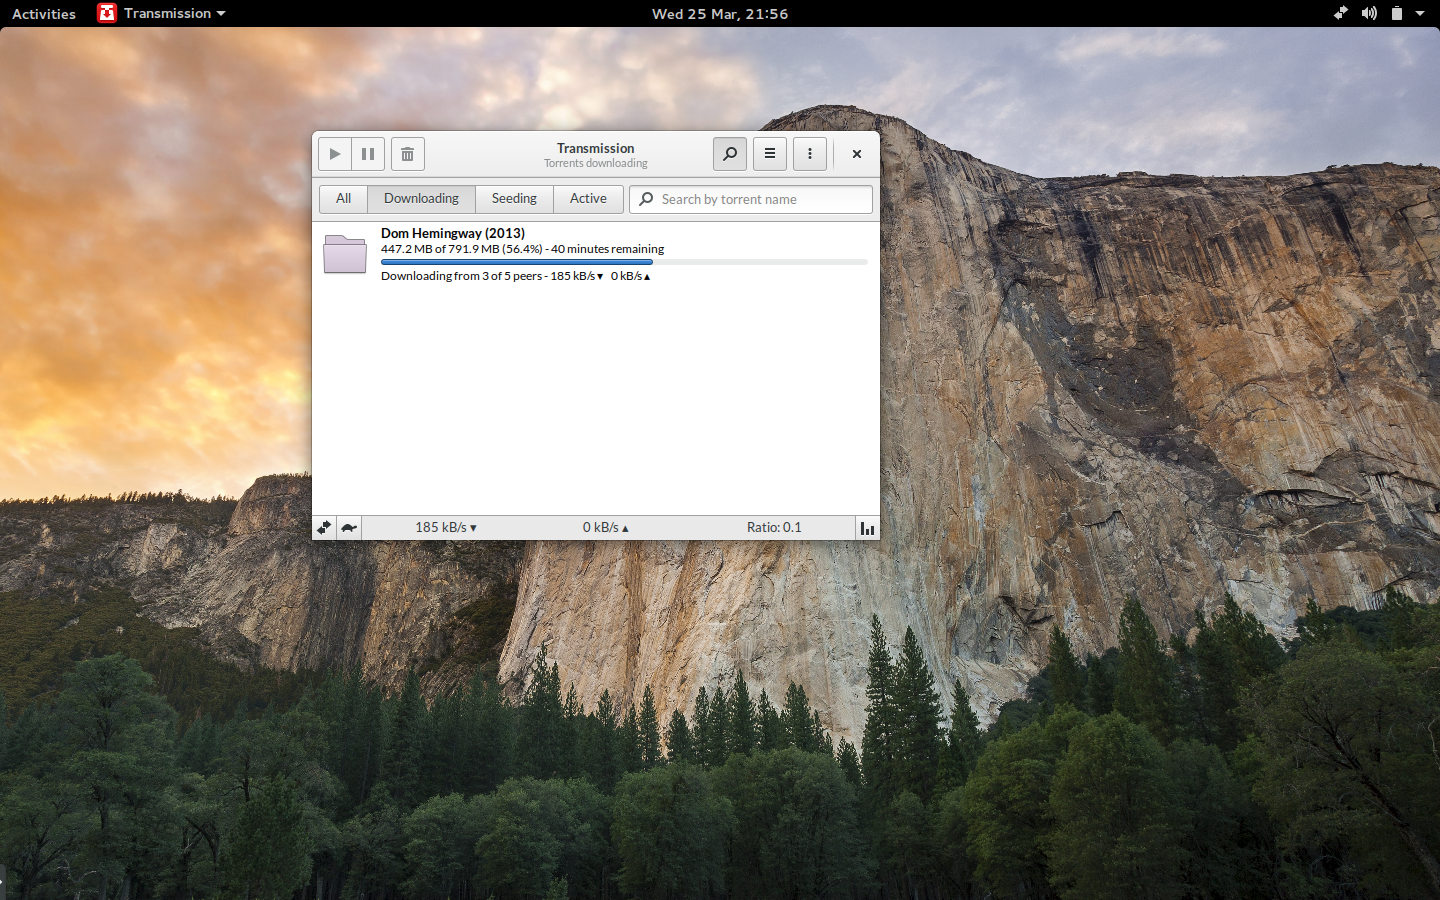
\includegraphics[width=\textwidth]{image/transmission-gtk3-main.png}
    \label{transmission-prototype}
    \fonte{Do Autor (2015)}
  \end{center}
\end{figure}

Verificou-se que o embasamento nos dados evolutivos das aplicações centrais do
GNOME foi de grande utilidade para compreender o processo de redesign dos
aplicativos desta plataforma, possibilitando e facilitando a geração das
propostas de redesign do \textit{Transmission}.

\subsection{Percepções do processo de transição das aplicações centrais}

Durante o processo de análise longitudinal percebeu-se uma tendencia clara de
redução da razão área útil vs controles em todas aplicações centrais analisadas.
Também foi possível perceber a padronização da razão na versão 3.16 de todas as
aplicações. A \autoref{workarea-vs-chrome} apresenta as razões área útil vs
controles calculadas, enquanto a figura \autoref{coreapps-workarea-vs-chrome}
ilustra o processo de aquisição.

\begin{table}[htb]
\ibgetab{
  \caption{Área útil vs Controles}
  \label{workarea-vs-chrome}
}{
    \begin{tabular}{ | l | l | l | } 
    \hline
    Aplicação & Versão 3.6 & Versão 3.16 \\
    \hline
    \textit{Nautilus}  & 0.17       & 0.07 \\
    \textit{Evince}    & 0.18       & 0.07 \\
    \textit{Gedit}     & 0.16       & 0.07 \\
    \hline
    \end{tabular}
}{
  \fonte{Do Autor (2015)}
}
\end{table}

\begin{figure}[!ht]
  \begin{center}
    \caption{\textbf{Aquisição das razões área útil vs controles}}
    \includegraphics [width=\textwidth]{image/coreapps-workarea-chrome-ratio.eps}
    \label{coreapps-workarea-vs-chrome}
    \fonte{Do Autor (2015)}
  \end{center}
\end{figure}


A tendência de redução desta razão se repete na remodelagem da forma e função de
vários widgets, uma clara influência de ambos design de usabilidade e da redução
de espaço vertical, visto a padronização de resoluções baseados na razão 16:9
(720p, 1080p, etc).

Falando específicamente sobre os elementos de interface, um dos elementos mais
comuns de um ambiente gráfico baseado em janelas é a barra de título, por onde o
usuário pode mover a janela no espaço de trabalho. Até então, no GNOME,
desenvolvedores tinham pouco ou nenhum controle sobre elas por questões de
compatibilidade de software.

Com a introdução do conceito de \textit{Header Bar}, as antigas barras de título
passam a acomodar botões, caixas de texto, sliders, etc, substituindo as barras
de ferramentas, antes encontradas comumente abaixo de menus ou das barras de
título, conforme a \autoref{toolbar-positioning}.

\begin{figure}[!ht]
  \begin{center}
    \caption{\textbf{Barra de Ferramentas no \textit{Evince} e \textit{Gedit} 3.6}}
    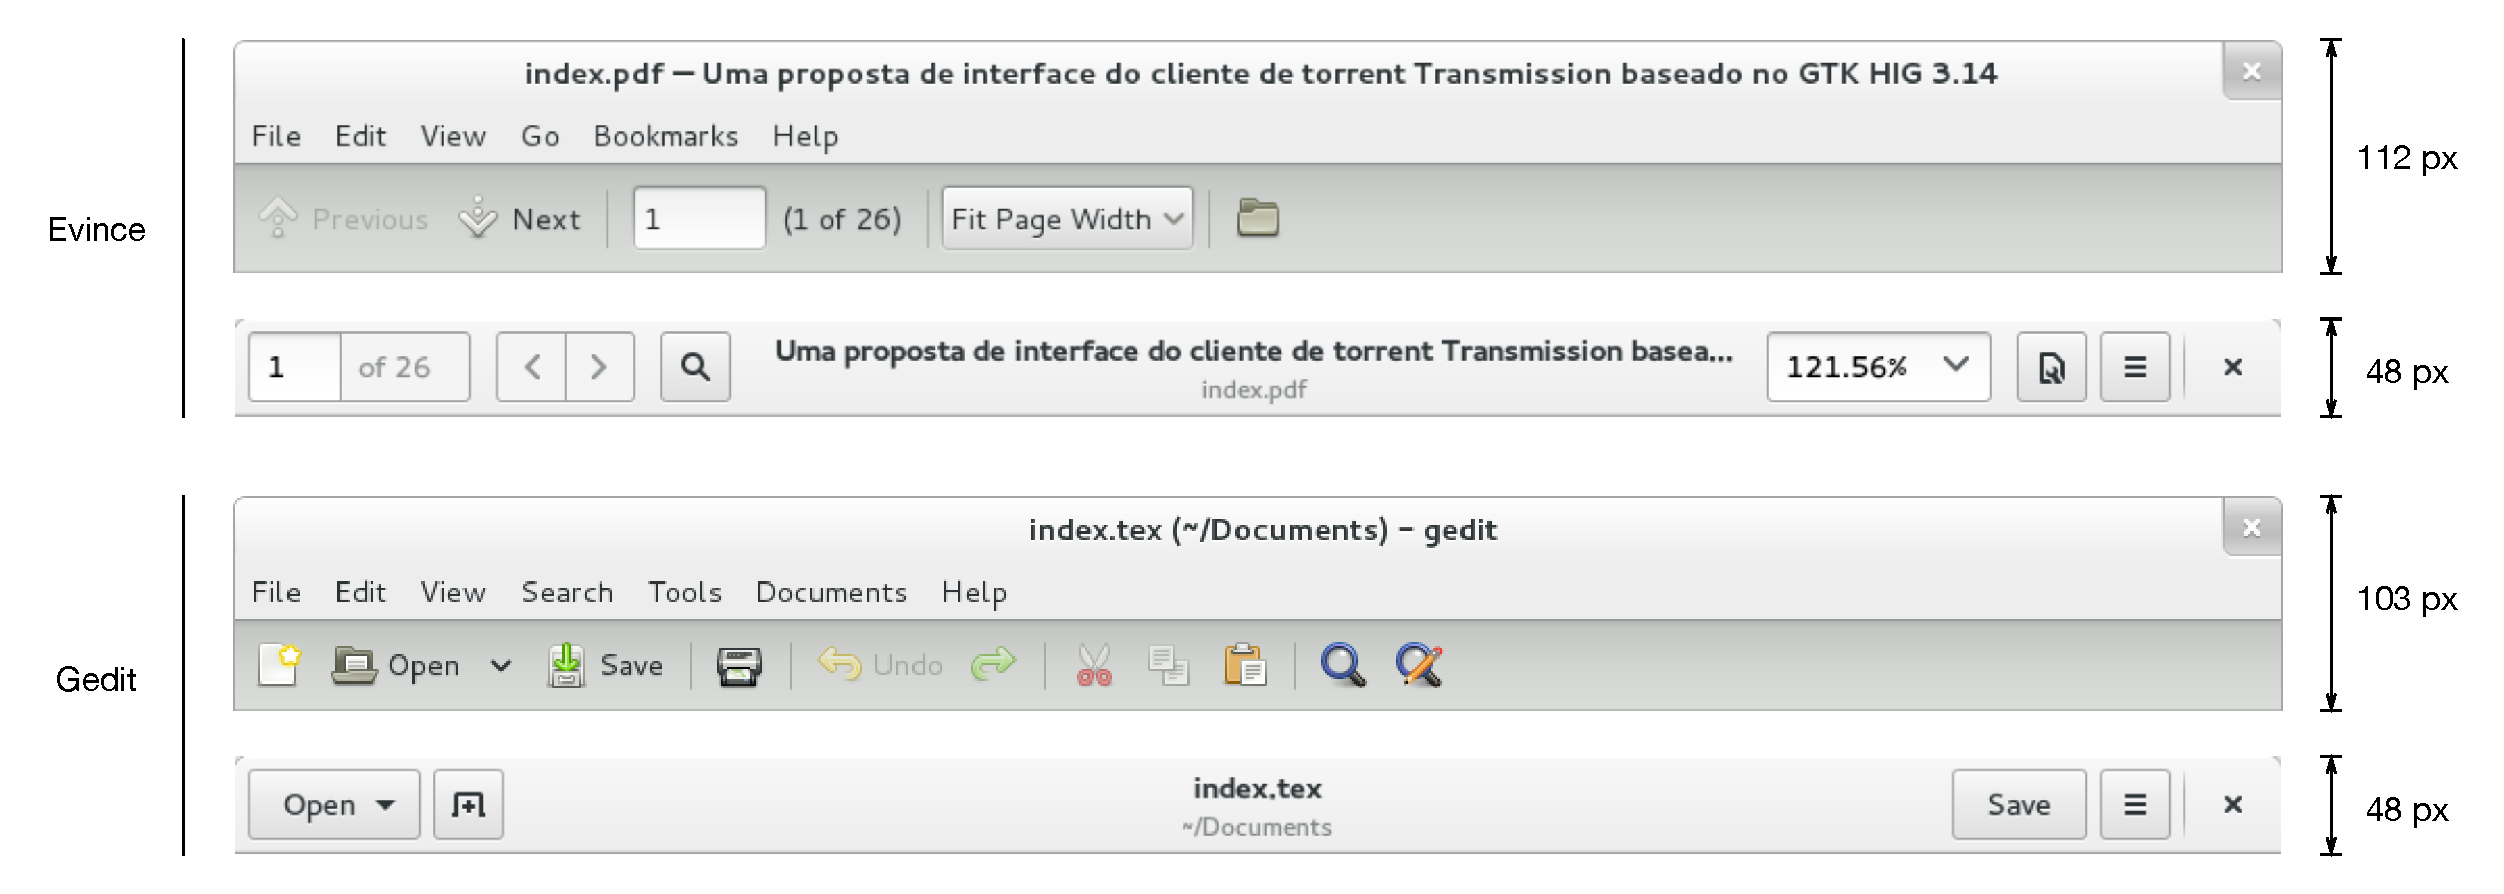
\includegraphics [width=\textwidth]{image/toolbar-headerbar-comparison.eps}
    \fonte{Do Autor (2015)}
    \label{toolbar-positioning}
  \end{center}
\end{figure}

Constatou-se que, dentre as aplicações analisadas na versão 3.6, o
\textit{Nautilus} foi a mais avançada em relação aos padrões de design definidos
pelo HIG, antes mesmo deste guia ser publicado, através da pré-implementação de
uma \textit{Header Bar}, abaixo da barra de título, evidênciando a
experimentação progressiva dos novos padrões antes de uma aplicação geral.

Outra mudança notável foi a transição da barra de menus, quais ações foram
dissolvidas através de um ou mais widgets na janela do programa (sendo grande
maioria na \textit{Header Bar}), nas ações pertinentes a janela, e em um menu de
aplicação, para ações pertinentes ao programa (Abrir, Sobre, Sair). A  
\autoref{rip-menubar} apresenta um mapeamento aproximado das ações da barra de 
menus do \textit{Evince} 3.6 para o 3.16.

\begin{figure}[!ht]
  \begin{center}
    \caption{\textbf{Mapeamento de menu no \textit{Evince}}}
    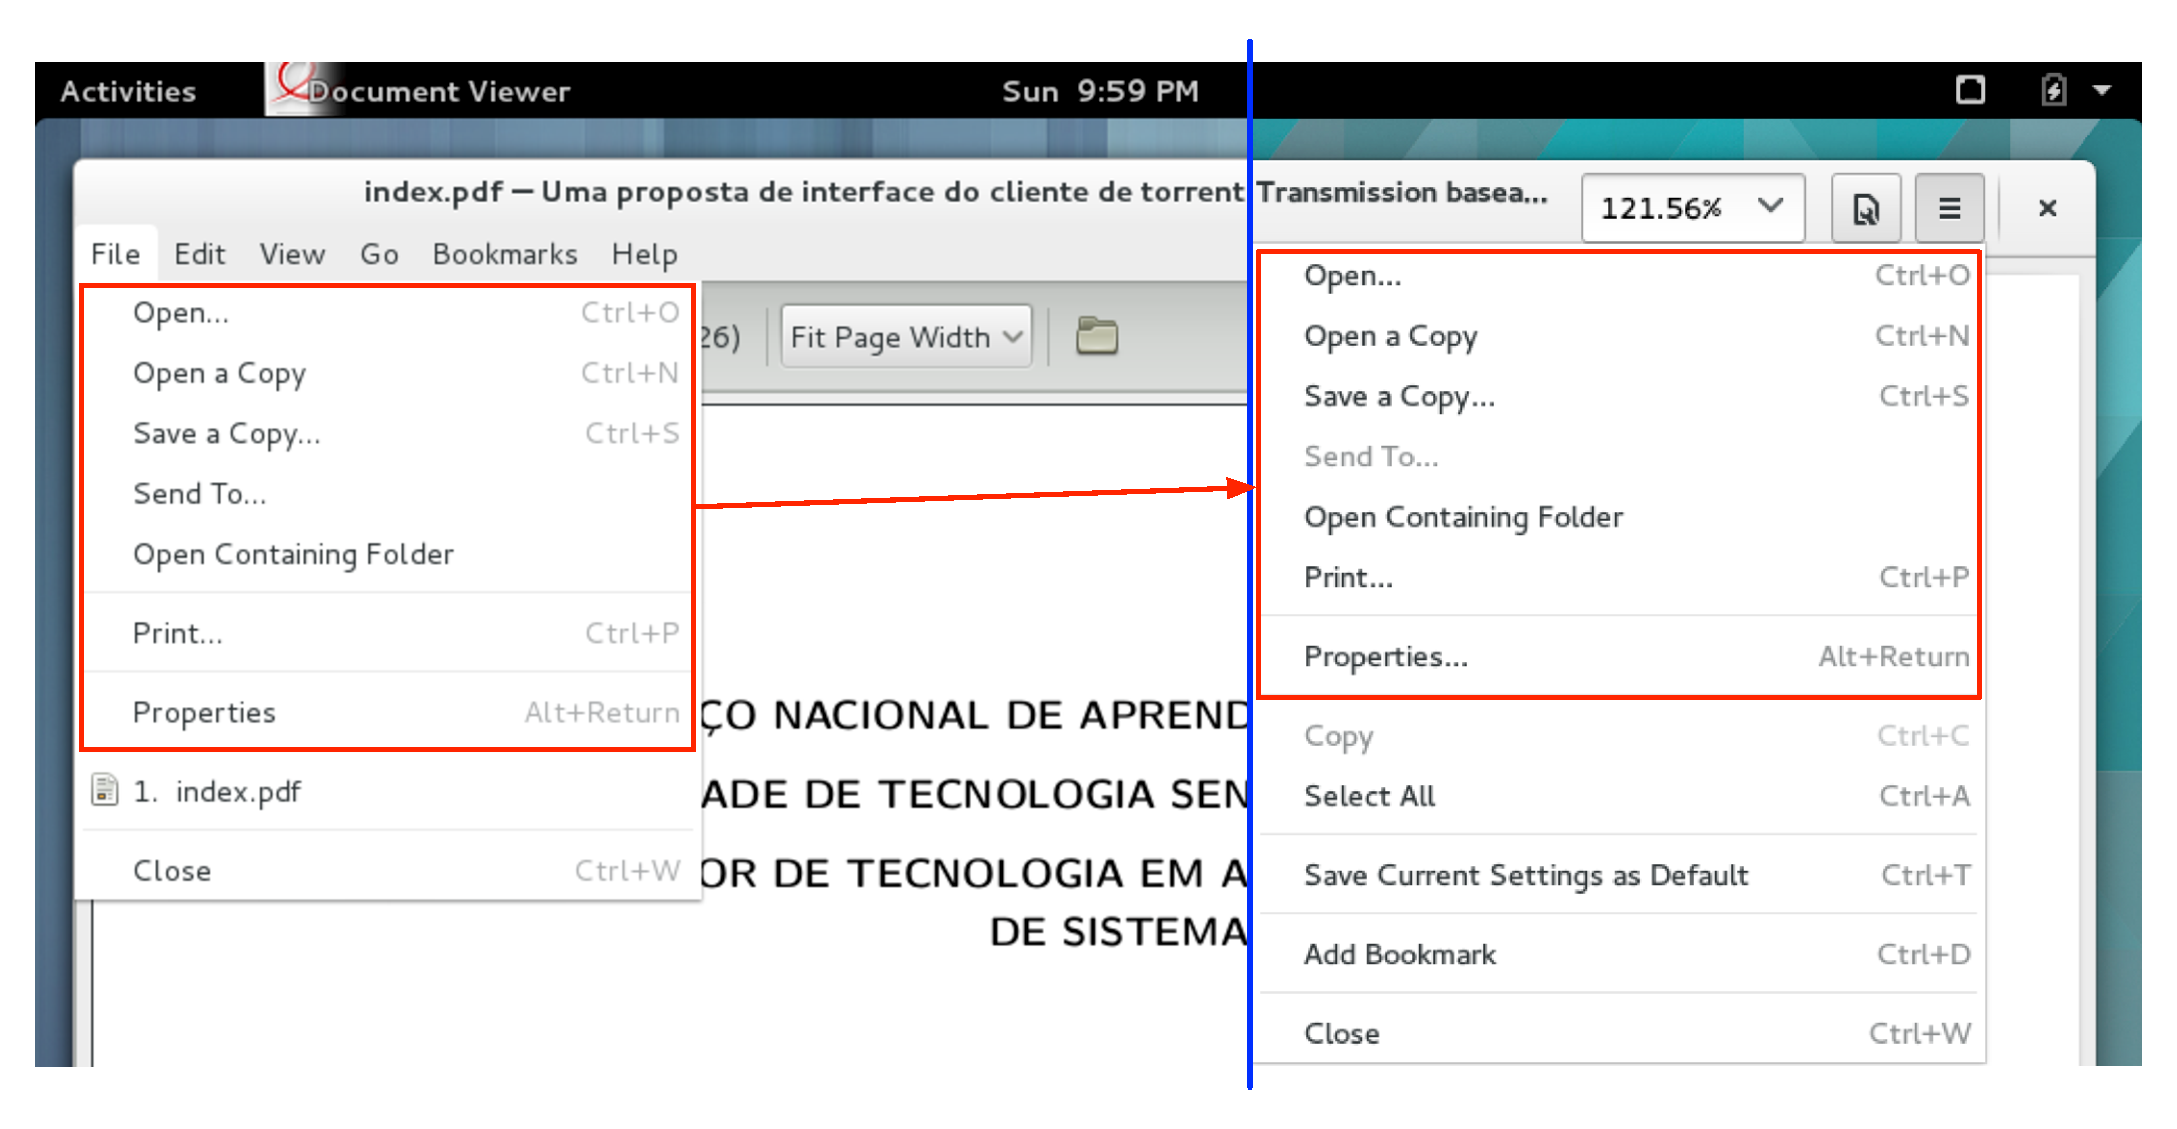
\includegraphics [width=\textwidth]{image/evince-menubar-mapping.eps}
    \fonte{Do Autor (2015)}
    \label{rip-menubar}
  \end{center}
\end{figure}

A utilização do \textit{Revealer} em ambos \textit{Nautilus} e \textit{Evince}
também demonstrou-se eficaz como técnica para redução de espaço vertical e
aumento da área útil de ambos programas, através da exibição transiente da caixa
de busca, alternável pelo botão lupa no \textit{Header Bar}.

O \textit{Popover}, um elemento de interface introduzido no HIG 3.12, é uma
visão transiente e flutuante que permitite adicionar menus, listas e widgets
variados em seu interior, e é comumente usado como parte de menus ou menus de
contexto. Sua utilização foi observada em diversos pontos, inclusive como
coadjuvante na transição da barra de menus em todas aplicações analisadas.

\section{Processo de redesign da interface do textit{Transmission}}

Em relação a utilização do \textit{Transmission} após o contato com as
aplicações centrais do GNOME 3.16 fica claro, logo na primeira utilização, que
sua interface não adere aos padrões incluídos no HIG, e se mostra completamente
desatualizada.

Foi possível, através da análise da transição das aplicações centrais do GNOME,
compilar uma série de modificações que podem ser aplicadas em prol da melhoria
da compatibilidade da interface do \textit{Transmission} com a experiência
GNOME, quais serão apresentadas a seguir.

\subsection{Header Bar}

A implementação da \textit{Header Bar} no \textit{Transmission} foi efetivada
através da dissolução das ações encontradas em ambas barra de ferramentas e
menus em botões. As ações da barra de menus foram separadas em duas categorias
de menu: Ações pertinentes ao programa e ações pertinentes a transferência
selecionada, posicionados da direita para a esquerda, respectivamente, conforme
indicado pelo HIG.

A \autoref{header-bar-transition} apresenta um paralelo entre a interface antiga
e a interface proposta, relacionando através de marcação em cores as transições
efetuadas. Os botões sensíveis a selecão (Iniciar, Parar e Remover) puderam ser
mantidos com seu comportamento original.

\begin{figure}[!ht]
  \begin{center}
    \caption{\textbf{Transição da \textit{Header Bar}}}
    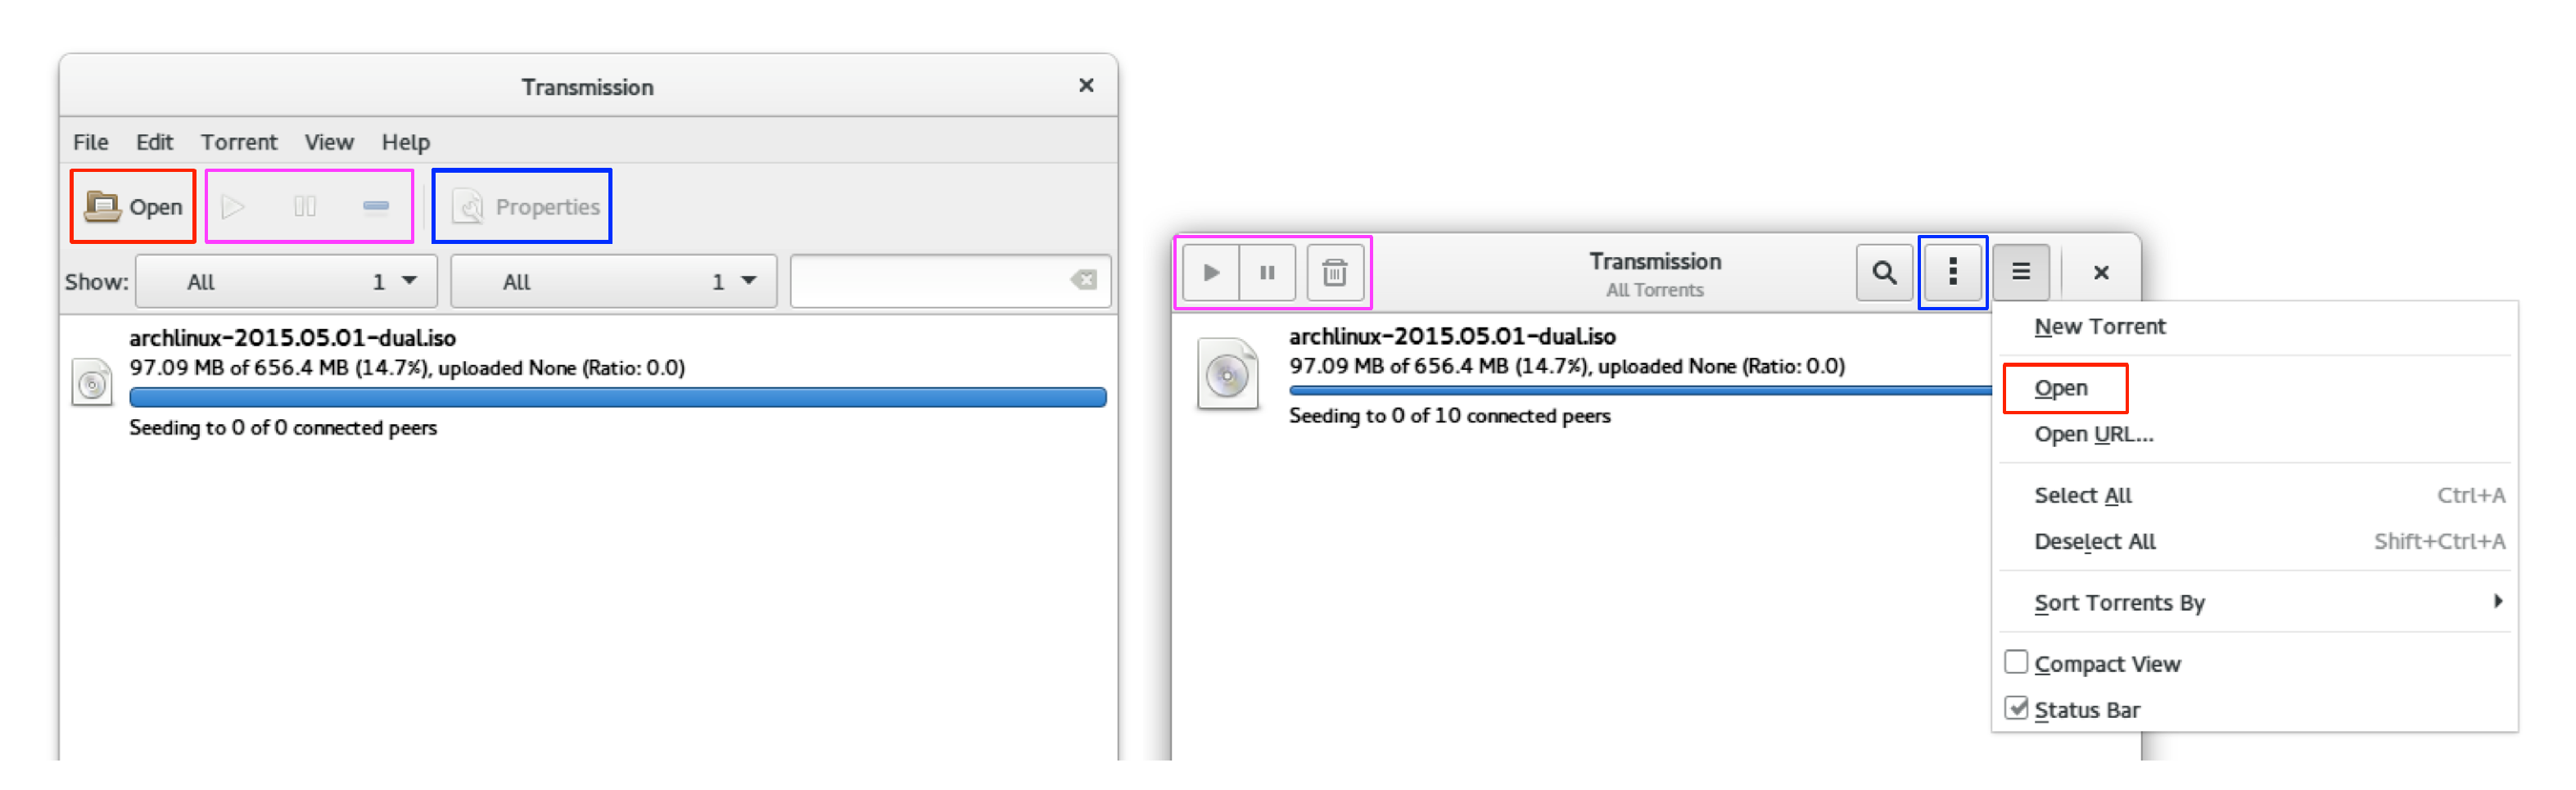
\includegraphics [width=\textwidth]{image/header-bar-transition.eps}
    \label{header-bar-transition}
    \fonte{Do Autor (2015)}
  \end{center}
\end{figure}

Pela natureza compacta da janela do \textit{Transmission} e pelo
compartilhamento do espaço disponível na \textit{Header Bar} pelos botões de
ação e título da aplicação, a adição excessiva de botões pode suprimir o título
da janela, e a presença de um número diferente de botões no lados direito e
esquerdo pode fazer parecer com que o título não esteja centralizado, causando
desconforto visual. Por este motivo os botões ``Properties'' e ``Open'' foram
migrados para os menus, sendo este movido para o menu de janela e aquele para o
menu de seleção.

\subsection{Barra de Filtros}

Seguindo a implementação utilizada no \textit{Evince} e \textit{Nautilus}, os
filtros de atividade foram movidos juntamente a caixa de busca textual para um
\textit{Revealer}, ativado através do botão com ícone de lupa, destacado na
\autoref{revealer}.

\begin{figure}[!ht]
  \begin{center}
    \caption{\textbf{Filtros retráteis através do uso de um Revealer}}
    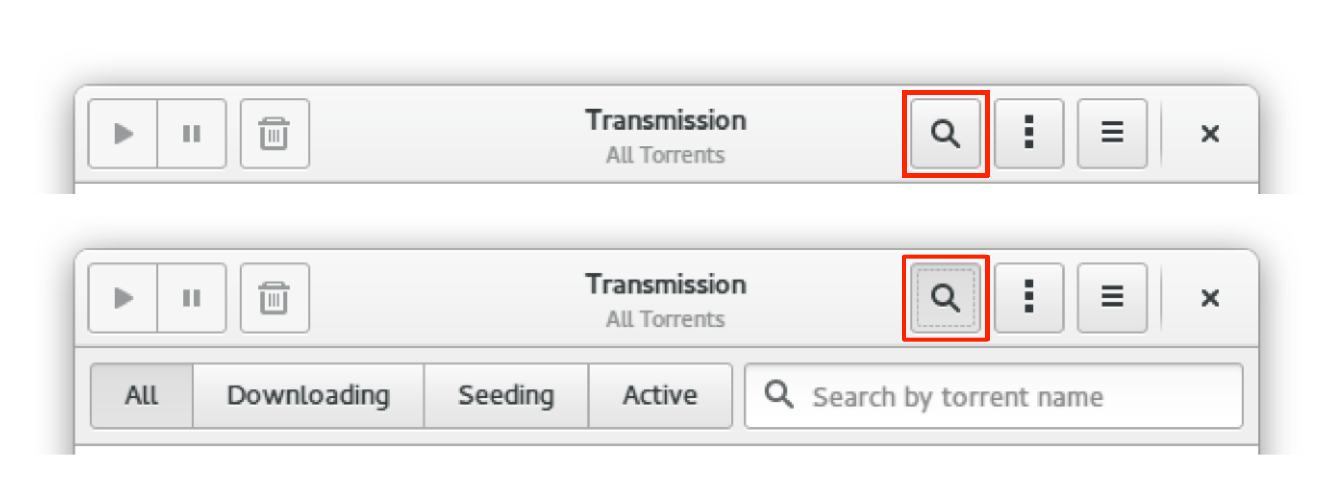
\includegraphics [width=\textwidth]{image/revealer.eps}
    \label{revealer}
    \fonte{Do Autor (2015)}
  \end{center}
\end{figure}

Na versão original do \textit{Transmission}, além do filtro textual, existem
dois tipos de filtros adicionais: Por estado (Recebendo, Transmitindo, Parado) e
por \textit{tracker} (Servidores que auxiliam a troca de arquivos). Por questões
de poupança de espaço a funcionalidade de filtragem por \textit{tracker} foi
deliberadamente removida.

\subsection{Limites Globais de Upload/Download}

Utilizando-se de um padrão de design já existente na interface gráfica do
\textit{Transmission} para Apple Mac OS X como fonte de inspiração, foi
implementada a configuração de limite de velocidade global utilizando um
\textit{Popover}, substituindo o extenso menu existente anteriormente, de forma
a permitir uma configuração fácil e rápida com poucos cliques. A
\autoref{global-limits-transition} apresenta um paralelo entre a implementação
original, a fonte de inspiração e o resultado derivado.

\begin{figure}[!ht]
  \begin{center}
    \caption{\textbf{Transição do menu de limites globais}}
    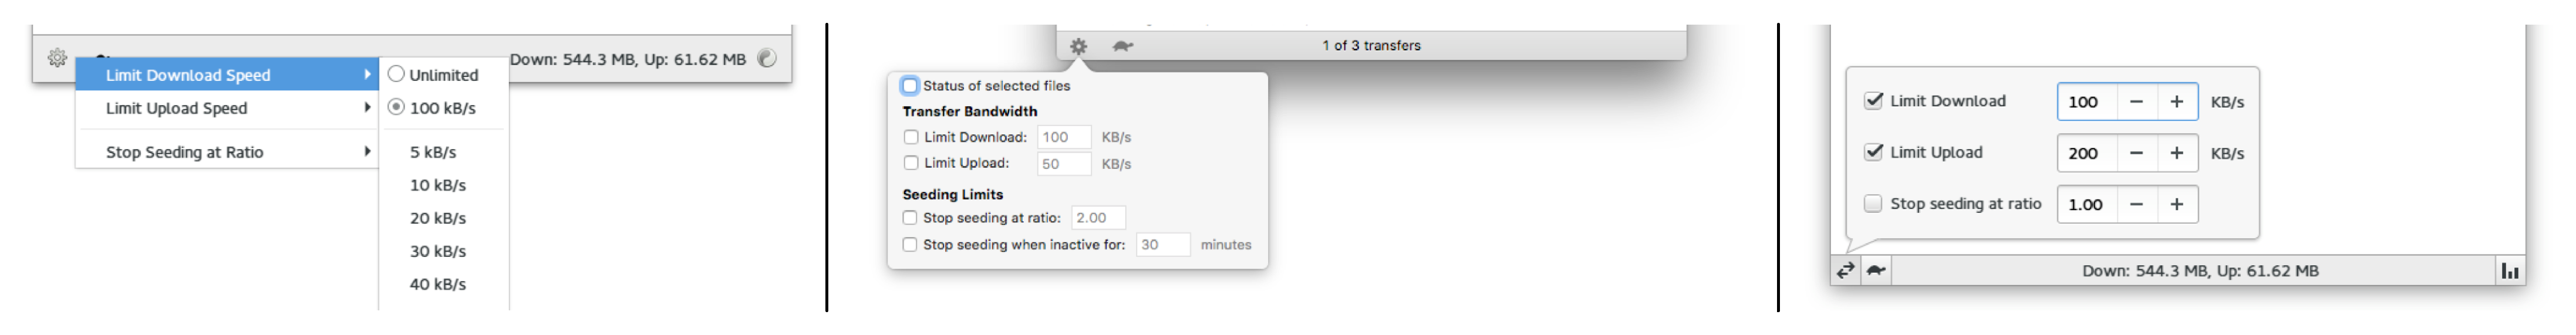
\includegraphics [width=\textwidth]{image/global-limits-transition.eps}
    \label{global-limits-transition}
    \fonte{Do Autor (2015)}
  \end{center}
\end{figure}

\subsection{Barra de Estado}

Inspirada na barra de estado do \textit{Gedit}, de altura compacta, e
utilizando-se das facilidades do GTK+ 3, todos os botões da barra de estado
foram implementados utilizando ícones simbólicos, de forma a se adaptarem a
temas claros e escuros (ilustrado na \autoref{status-bar}). Para implementar as
opções de visualização das estatísticas (último botão da esquerda para a
direita) foi utilizado um \textit{Popover}.

\begin{figure}[!ht]
  \begin{center}
    \caption{\textbf{Ícones simbólicos na barra de estado}}
    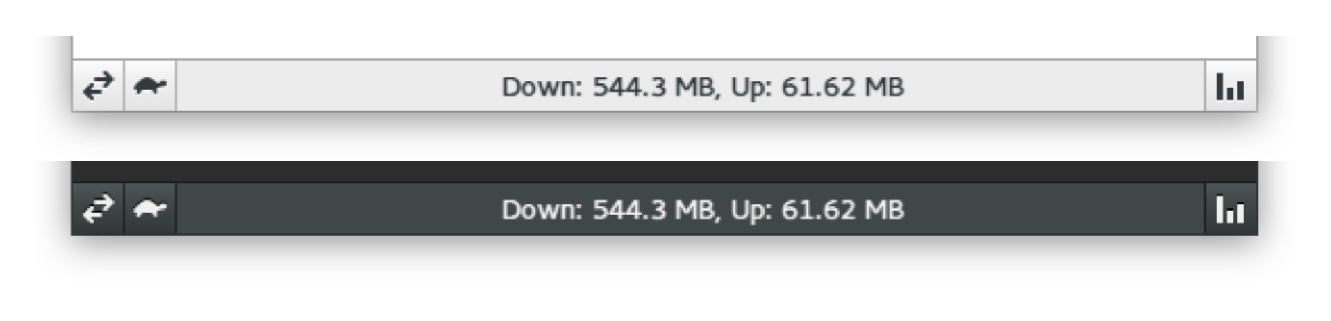
\includegraphics [width=\textwidth]{image/status-bar.eps}
    \label{status-bar}
    \fonte{Do Autor (2015)}
  \end{center}
\end{figure}
